\que{Задача о сдвиге прямоугольного бруса.}

Рассмотрим тело $V$ в форме параллелепипеда, где $l_i$ длины его ребер. 

Выберем ДСК $O\bar{\mathbf{e}}_i$ таким образом, чтобы боковые поверхности $V$ имели следующее уравнение:
\begin{align*}
	x^i &= \pm \frac{l_i}{2}; \\
	\tau &= \frac{F^j_r}{\Sigma_j} = \sigma_{rj}.
\end{align*}
Где 
$F^j_r$ --- касательная компонента (сила)ж

$r$ --- площадка, на которую действует сила;

$j$ --- проекция в направлениях.

Изобразим сечение одной плоскости прямоугольного параллелепипеда:

% TODO: \usepackage{graphicx} required
\begin{figure}[H]
	\centering
	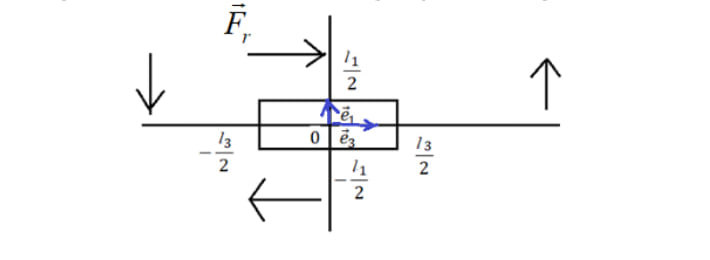
\includegraphics[width=0.7\linewidth]{semester8/img/27}
	\caption{}
	\label{fig:27}
\end{figure}

Пусть на боковых поверхностях $x_3 = \pm \frac{l_3}{2}$ и $x_1 = \pm \frac{l_1}{2}$ заданы касательные константы, вектор напряжений, а поверхность $x_2 = \pm \frac{l_2}{2}$ --- свободны. 

\begin{enumerate}
	\item На $x_1 = \pm \frac{l_1}{2}, \quad \mathbf{t}_{n_e} = \mathbf{n} \cdot \sigma = \tau \mathbf{b}_3 \quad (\sigma_{13} = \tau, \sigma_{12} = 0, \sigma_{11} = 0)$
		
	\item На $x_3 = \pm \frac{l_3}{2}, \quad \mathbf{t}_{n_e} = \mathbf{n} \cdot \sigma = \tau \mathbf{b}_1 \quad (\sigma_{13} = \tau, \sigma_{23} = 0, \sigma_{33} = 0)$
	
	\item На $x_2 = \pm \frac{l_2}{2}, \quad \mathbf{t}_{n_e} = \mathbf{n} \cdot \sigma = 0 \quad (\sigma_{12} = \tau, \sigma_{23} = 0, \sigma_{22} = 0)$
\end{enumerate}

Если массовых сил нет $\vec{f} = 0$ и процессы деформирования квазистатические, то напряжение, являющиеся решением и ГУ, имеет следующий вид:
\boxed{\sigma_{13} = \tau = \mathrm{const}}, а остальные \boxed{\sigma_{ij} \equiv 0} $\forall \vec{x} \in V$
\begin{itemize}
	\item Деформацию вычисляем:
	\begin{equation*}
		\varepsilon_{ij} = \Pi_{ijkl} \sigma_{kl} = 2 \Pi_{ij13} \tau
	\end{equation*}
	
	\item Для ортотропных сред:
	\begin{equation*}
		\varepsilon_{13} = 2 \Pi_{1313} \tau \Rightarrow \varepsilon_{13} = \frac{1}{2 G_{13} \tau}
	\end{equation*}
	
	\item Измеряя $\varepsilon_{13}$ и $\tau$ находим модуль сдвига. 
	\begin{equation*}
		\boxed{G_{13} = \frac{\tau}{2 \varepsilon_{13}}.}
	\end{equation*}
\end{itemize}

Для ортотропных сред задача о сдвиге используется для определения $G_{12}$, $G_{13}$ и $G_{23}$.

Для нахождения перемещений используем формулу Чезаро после жёсткого защемления одной точки, например, $\mathbf{x}_0 = 0$:
\begin{equation*}
	\boxed{\mathbf{u} = \varepsilon \cdot \mathbf{x}}, \quad \boxed{u_i = \varepsilon_{ij} \cdot x_{j}}
\end{equation*} 